% Updated report from the completed ten-seed controlled study.
\RequirePackage{fix-cm}
\documentclass[12pt]{article}
\usepackage{latex_template,iftex}
\ifPDFTeX\usepackage{times}\else
\usepackage{fontspec}
\IfFontExistsTF{Times New Roman}{\setmainfont{Times New Roman}}{\setmainfont{TeX Gyre Termes}}
\fi
\usepackage{amsmath,amssymb,booktabs,graphicx,hyperref,float,placeins,array}
\hypersetup{hidelinks}
\urlstyle{same}
\makeatletter
\renewcommand{\normalsize}{%
\@setfontsize\normalsize{12pt}{14.5pt}%
\abovedisplayskip 6pt plus 2pt minus 2pt
\belowdisplayskip 6pt plus 2pt minus 2pt
\abovedisplayshortskip 3pt plus 1pt minus 1pt
\belowdisplayshortskip 3pt plus 1pt minus 1pt}
\renewcommand{\small}{\@setfontsize\small{10pt}{12pt}}
\makeatother
\normalsize\raggedbottom
\setlength{\textfloatsep}{9pt plus 2pt minus 2pt}
\setlength{\intextsep}{8pt plus 2pt minus 2pt}
\setlength{\abovecaptionskip}{4pt}
\setlength{\belowcaptionskip}{3pt}
\title{\fontsize{14}{17}\selectfont Learning with Class-Conditional Label Noise:\\
Transition Estimation and Controlled Classifier Comparisons}
\author{\normalfont\fontsize{12}{14.5}\selectfont
Group 39\\
\normalfont Subaial Awan --- 560795376 --- sawa3871\\
\normalfont Nihira Sharma --- 530784106 --- nsha0877\\
\normalfont Vaibhavi Shivanna --- 560394478 --- vshi0379}
\nipsfinalcopy
\newcommand{\FMaUniformError}{0.8602}
\newcommand{\FMaUniformRelative}{0.387}
\newcommand{\FMaBudgetDiff}{-0.28}
\newcommand{\FMaBudgetP}{0.00073}
\newcommand{\FMaBudgetLow}{-0.37}
\newcommand{\FMaBudgetHigh}{-0.18}
\newcommand{\FMaRevisionDiff}{0.00}
\newcommand{\FMaRevisionP}{1.00000}
\newcommand{\FMaRevisionLow}{-0.00}
\newcommand{\FMaRevisionHigh}{0.01}
\newcommand{\FMbUniformError}{0.1414}
\newcommand{\FMbUniformRelative}{0.442}
\newcommand{\FMbBudgetDiff}{0.18}
\newcommand{\FMbBudgetP}{1.00000}
\newcommand{\FMbBudgetLow}{-0.57}
\newcommand{\FMbBudgetHigh}{0.92}
\newcommand{\FMbRevisionDiff}{0.17}
\newcommand{\FMbRevisionP}{0.27946}
\newcommand{\FMbRevisionLow}{-0.01}
\newcommand{\FMbRevisionHigh}{0.35}
\newcommand{\CIFBudgetDiff}{-0.07}
\newcommand{\CIFBudgetP}{1.00000}
\newcommand{\CIFBudgetLow}{-2.17}
\newcommand{\CIFBudgetHigh}{2.03}
\newcommand{\CIFRevisionDiff}{0.48}
\newcommand{\CIFRevisionP}{0.32810}
\newcommand{\CIFRevisionLow}{-0.07}
\newcommand{\CIFRevisionHigh}{1.03}
\newcommand{\CifarClassifierMean}{68.57}
\newcommand{\CifarClassifierSD}{1.21}
\newcommand{\CifarEstimatorMean}{68.89}
\newcommand{\CifarEstimatorSD}{3.37}
\newcommand{\SupplementRuntime}{146.09 minutes}

\begin{document}
\maketitle
\begin{abstract}
We study three-class image classification with class-conditional label noise using Forward correction and Reweight-R, an importance-weighting/transition-revision hybrid. Supplied FashionMNIST transitions and split-specific CIFAR estimates support ten repeated holdouts. To distinguish method effects from training budget, we add a cross-entropy baseline, epoch-matched Forward training and a fixed-matrix continuation from the same checkpoint and random state. Epoch matching favors Forward on FashionMNIST0.3 (99.08\% versus 98.80\%); controlled revision gains are not established after multiplicity adjustment. We also test anchor counts, noisy-label temperature calibration and CIFAR randomness controls. The report presents the methods, controlled results, estimator diagnostics and reproducibility limitations.
\end{abstract}

\section{Introduction}
Large image collections often obtain labels through crowdsourcing or automatic annotation. Re-annotating every example can require substantial time and expertise, restricting dataset size and coverage \cite{rolnick2017,xia2019}. A classifier trained on corrupted labels can learn the annotation process rather than the intended categories; systematic class-dependent errors can also damage particular classes while aggregate accuracy conceals them. Correction is useful when relabelling is unavailable and the corruption process has a plausible model. It is not universally preferable to obtaining better labels: incorrect noise assumptions can introduce further bias.

We train and validate on noisy labels and evaluate on clean test labels. We compare Forward correction with a T-Revision-inspired hybrid and assess transition estimation. Controlled experiments distinguish optimization budget from matrix revision and probe classifier/estimator randomness on CIFAR. Clean-label evaluations follow fitting and checkpoint selection.

\section{Related work}
Noise-aware methods differ in their assumptions and guarantees. Natarajan et al.~\cite{natarajan2013} construct unbiased corrected losses given suitable noise information; their binary results do not directly establish multiclass CNN performance. Patrini et al.~\cite{patrini2017} distinguish Backward loss correction from Forward probability correction. Backward offers a clean-risk interpretation but inversion can amplify matrix error. Forward avoids explicit inversion and has a population recovery argument under a correct nonsingular transition and suitable loss/model assumptions; finite-sample optimization remains a separate issue.

Importance reweighting retains familiar surrogate losses but requires reliable posterior ratios \cite{liu2016}. Xia et al.~\cite{xia2019} jointly revise an initial transition, reducing reliance on exact anchors at the cost of additional optimization and identification assumptions. Our final stage uses Forward loss instead of their original objective, so its guarantees cannot simply be transferred. Learned transition correction is our extension of the supplied Weeks~8--9 Forward/reweighting/anchor formulations.

Matrix-based correction retains all examples and avoids a second network, but depends on transition estimation when $T$ is unknown; Co-teaching instead depends on its example-selection and retention policy \cite{han2018coteaching}. Ordinary networks can themselves tolerate some noise \cite{rolnick2017}, motivating a cross-entropy baseline. Temperature scaling targets confidence calibration \cite{guo2017}; we adapt it to the \emph{noisy} posterior and test rather than assume that better global calibration improves anchor estimates.

\section{Methods}
\subsection{Noise model and shared classifier}
For image $X$, clean label $Y$ and noisy label $S\in\{0,1,2\}$, define $T_{ij}=P(S=j\mid Y=i,X)=P(S=j\mid Y=i)$. Rows index clean classes, columns noisy classes, and $\sum_jT_{ij}=1$. Row-vector posteriors obey $q(x)=p(x)T$, where $p_i=P(Y=i\mid x)$ and $q_j=P(S=j\mid x)$. Clean predictions are $\arg\max_i p_{\theta,i}(x)$. We use the supplied matrices directly:
\begin{equation}
T_{0.3}=\begin{bmatrix}.7&.3&0\\0&.7&.3\\.3&0&.7\end{bmatrix},\qquad
T_{0.6}=\begin{bmatrix}.4&.3&.3\\.3&.4&.3\\.3&.3&.4\end{bmatrix}.
\label{eq:known}
\end{equation}
Thus clean class 0 flips to noisy class 1 with probability 0.3 in $T_{0.3}$. The lecture's opposite indexing is the transpose; all our components consistently use clean-class rows.

The shared CNN has two $3\times3$ convolutions (padding 1; 16/32 channels), each with batch normalization, ReLU and $2\times2$ max pooling, followed by adaptive $4\times4$ pooling, dropout 0.25 and fully connected widths $512\rightarrow64\rightarrow3$. This controls capacity differences and limits CPU cost. Batches contain 128 examples. Adam uses network weight decay $10^{-4}$; dropout and validation-selected checkpoints also limit overfitting without guaranteeing its elimination.

\subsection{Forward and Reweight-R objectives}
Forward minimizes
\begin{equation}
\mathcal L_{\rm F}(\theta;T)=-\frac1n\sum_r\log([p_\theta(X_r)T]_{S_r}+\epsilon),\qquad\epsilon=10^{-7}.
\label{eq:forward}
\end{equation}
Ignoring the stabilizer, population minimization matches the true noisy posterior. A correct nonsingular $T$ identifies the clean posterior, but this does not guarantee that a finite CNN reaches the optimum. Forward uses Adam at initial learning rate $10^{-3}$ with a cosine schedule over its four or fourteen epochs.

Reweight-R uses two noisy-label cross-entropy warm-up epochs and four fixed-matrix epochs of
\begin{equation}
\mathcal L_{\rm R}(\theta;T)=\frac1n\sum_r\operatorname{sg}\!\left(
\frac{p_{\theta,S_r}(X_r)}{[p_\theta(X_r)T]_{S_r}+\epsilon}\right)[-\log p_{\theta,S_r}(X_r)].
\label{eq:reweight}
\end{equation}
Here $\operatorname{sg}$ stops gradients through the recomputed weight. With true fixed ratios, weighted noisy risk equals clean risk on suitable support. Plug-in ratios do not inherit that guarantee: detachment retains $\beta\nabla\ell$ while omitting $\ell\nabla\beta$ from the full derivative of $\beta\ell$. Warm-up and fixed training each use a separate cosine schedule starting at $10^{-3}$.

For an idealized pointwise population argument, ignore $\epsilon$, assume positive posteriors and let $q^*=p^*T$. The detached update's expected logit gradient is
\begin{equation}
g_j=p_j\left(Z-\frac{q_j^*}{q_j}\right),\qquad
Z=\sum_s\frac{q_s^*p_s}{q_s},\quad q=pT.
\label{eq:stationary}
\end{equation}
If $g=0$ and every $p_j>0$, all ratios $q_j^*/q_j$ equal $Z$. Summing distributions gives $Z=1$, hence $q=q^*$ and, for nonsingular $T$, $p=p^*$. Thus the correct posterior is the unique interior stationary point in this idealization. This establishes neither global convergence nor a guarantee for shared finite CNN parameters, stabilization, estimated $T$ or joint revision.

\noindent\begin{minipage}{\linewidth}
The final eight epochs jointly update the network and $\Delta T$, initially zero, using Forward loss and the revised matrix
\begin{equation}
M_{ij}=\max(T_{ij}+\Delta T_{ij},0),\quad r_i=\sum_jM_{ij},\qquad
T'_{ij}=\begin{cases}M_{ij}/r_i,&r_i>0,\\T_{ij}/\sum_kT_{ik},&r_i=0.\end{cases}
\label{eq:revision}
\end{equation}
Clipping and row normalization include an input-row fallback. Revision uses fixed Adam learning rates $10^{-4}$ for both parameter groups; only network parameters receive weight decay.
\end{minipage}

\subsection{Selection, estimation and calibration}
Forward, warm-up and fixed reweighting restore the epoch with smallest noisy-validation Forward NLL under the input matrix. Revision retains the fixed-stage checkpoint as incumbent and accepts only lower validation NLL under a candidate $T'$. No clean test labels select checkpoints. Comparing candidate matrices through noisy likelihood does not establish better recovery of the corruption process.

A separate CNN trains for four epochs on noisy-label cross-entropy with the same optimizer settings, selecting by noisy-validation cross-entropy. For its noisy posterior $\hat q$, the estimator is
\begin{equation}
\mathcal A_i=\operatorname{TopK}_{r\in\mathcal D_{\rm tr}}\hat q_i(X_r),\qquad
\hat T_{ij}=\frac1k\sum_{r\in\mathcal A_i}\hat q_j(X_r).
\label{eq:anchor}
\end{equation}
Rows are normalized; ties are stable. At a pure clean anchor, $q_j(x)=T_{ij}$. Selecting high noisy-class confidence requires additional class alignment. A sufficient population condition is $T_{ii}>T_{ji}$ for every $j\ne i$, together with suitable pure anchors and accurate posterior estimates. These conditions are not verified for CIFAR. Only training examples are anchors. The canonical classifiers retain $k=10$; FashionMNIST uses supplied matrices, CIFAR uses each split's estimate.

For a calibration diagnostic, we split noisy validation equally into temperature-fit and check halves. A scalar $\tau\in[0.1,10]$ minimizes fit-half noisy NLL for $\operatorname{softmax}(f/\tau)$; its check-half NLL/ECE and calibrated $k=10$ matrix are evaluated separately. The check half is disjoint from temperature fitting, but previously participated in checkpoint selection. Calibrated matrices are diagnostic and do not replace the canonical classifier inputs.

\section{Experiments and results}
\subsection{Data, protocol and controlled comparisons}
FashionMNIST0.3/0.6 each contain 18,000 noisy grayscale $28\times28$ examples, split into 14,400 training and 3,600 validation examples. CIFAR has 15,000 RGB $32\times32$ examples, split into 12,000/3,000. Each clean test set contains 3,000 examples. FashionMNIST image arrays and clean test labels are identical across corruption settings; noisy training labels differ in both rate and structure.

Pixels are float32, divided by 255 and arranged channel-first. Per-channel standardization uses training-only mean/SD plus $10^{-6}$, preventing validation/test leakage and controlling input scale. No augmentation or cleaning is used. Ten random 80/20 holdouts (seeds 0--9) share splits, initialization policy and backbone between methods. These are repeated holdouts, not ten-fold cross-validation.

We add three training controls. \textbf{CE4} uses the four-epoch preliminary network's argmax directly, ignoring corruption. \textbf{F14} matches Reweight-R's fourteen total epochs; its cosine schedule spans fourteen epochs rather than the original four. \textbf{Fixed14} continues the exact six-epoch pre-revision checkpoint for eight Forward epochs with $\Delta T$ frozen at zero. It matches revision learning rate, optimizer, incumbent rule, minibatch order and dropout random state. Estimator and Reweight-R replays are checked against saved baseline matrices/predictions.

The anchor study changes only $k\in\{1,5,10,20\}$ on the same preliminary predictions. CIFAR diagnostics fix split 0 and either (a) its estimated matrix while varying classifier initialization/minibatch seed, or (b) classifier seed 0 while varying preliminary-estimator seed. Each arm has ten settings, including the shared reference seed 0. They probe sources of variability on one fold, not an additive variance decomposition.

Accuracy is clean-test top-1 percentage; descriptive SD uses denominator 10. Matrix error is $\|\hat T-T\|_F$. ECE uses fifteen equal-width confidence bins against \emph{noisy} check labels. Paired differences are expressed in percentage points (pp), with sample SD and individual 95\% $t_9$ intervals. Holm adjustment covers six prespecified contrasts: R14--F14 and R14--Fixed14 on three datasets. Clean test labels are used only after fitting.

\subsection{Epoch matching and revision isolation}
\begin{table}[H]\centering\fontsize{11}{13}\selectfont\setlength{\tabcolsep}{3pt}
\caption{Clean-test accuracy (\%), mean $\pm$ population SD over ten runs. FM denotes FashionMNIST. F4/F14 are Forward budgets; Fixed14 and R14 share the same six-epoch starting checkpoint.}
\label{tab:accuracy}\begin{tabular}{lccccc}
\toprule
Dataset & CE4 & F4 & F14 & Fixed14 & R14\\
\midrule
FM0.3 & $97.78\pm0.14$ & $98.51\pm0.11$ & $99.08\pm0.07$ & $98.80\pm0.13$ & $98.80\pm0.13$\\
FM0.6 & $94.04\pm1.37$ & $95.05\pm0.97$ & $95.03\pm1.32$ & $95.04\pm0.76$ & $95.21\pm0.66$\\
CIFAR & $64.15\pm3.57$ & $64.72\pm8.90$ & $65.75\pm8.67$ & $65.20\pm7.87$ & $65.68\pm7.55$\\
\bottomrule
\end{tabular}
\end{table}
Both corrected methods improve on CE4's FashionMNIST means. However, epoch matching reverses the original ranking at noise 0.3: F14 reaches $99.08\pm0.07\%$, exceeding R14's $98.80\pm0.13\%$. Extra Forward training does not consistently help at noise 0.6, where F4/F14 means are 95.05/95.03\%. On CIFAR, corrected means only modestly exceed CE4's 64.15\%, with substantially greater variability. Correction is therefore not uniformly more reliable than the simpler baseline.
\begin{table}[H]\centering\fontsize{11}{13}\selectfont\setlength{\tabcolsep}{4pt}
\caption{Paired R14-minus-control differences (pp), individual 95\% intervals and Holm-adjusted $p$-values across six contrasts.}
\label{tab:contrasts}\begin{tabular}{lcccc}
\toprule
Dataset & Control & $\Delta$ (pp) & 95\% CI & Holm $p$\\
\midrule
FM0.3 & F14 & $-0.277$ & $[-0.374,-0.179]$ & $0.00073$\\
FM0.3 & Fixed14 & $+0.003$ & $[-0.004,0.011]$ & $1.00000$\\
FM0.6 & F14 & $+0.177$ & $[-0.570,0.923]$ & $1.00000$\\
FM0.6 & Fixed14 & $+0.173$ & $[-0.005,0.352]$ & $0.27946$\\
CIFAR & F14 & $-0.070$ & $[-2.173,2.033]$ & $1.00000$\\
CIFAR & Fixed14 & $+0.480$ & $[-0.075,1.035]$ & $0.32810$\\
\bottomrule
\end{tabular}
\end{table}
Only F14's noise-0.3 advantage remains detectable after Holm adjustment ($p=0.00073$). Against Fixed14, R14 gains just 0.003, 0.173 and 0.480 percentage points respectively; adjusted $p$-values are 1.000, 0.279 and 0.328. These ten-run comparisons do not establish an independent revision benefit. At noise 0.3, eight runs have identical fixed/revised predictions, supporting extra optimization as the main explanation for the original R14 advantage over F4. Absence of significance does not establish equivalence.
\begin{figure}[H]\centering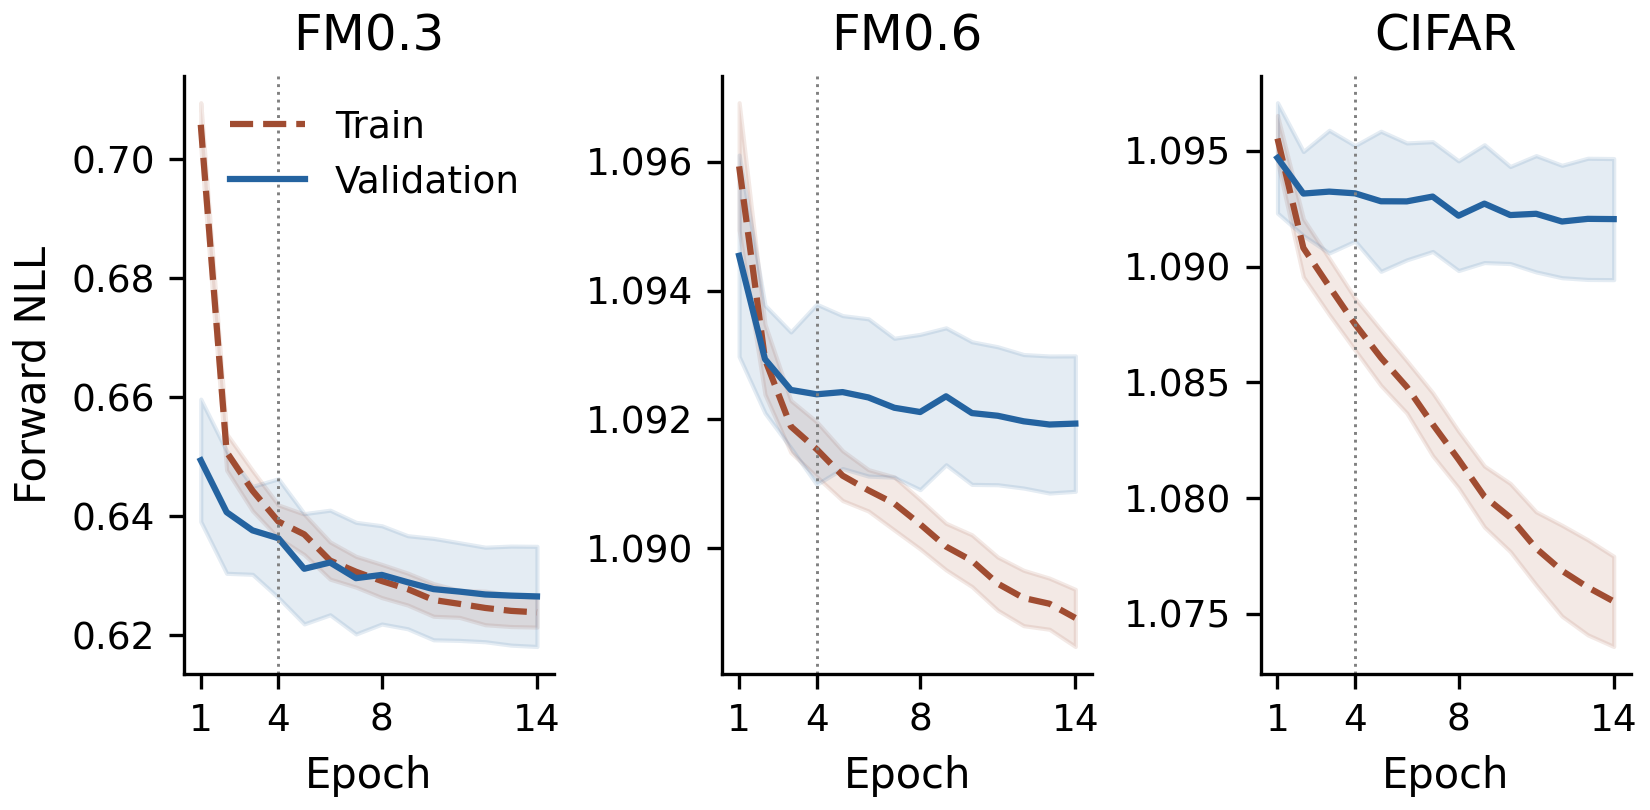
\includegraphics[width=\linewidth]{images/forward_learning_curves.png}
\caption{Forward14 train/validation NLL: means and population SD over ten runs. The vertical line marks epoch 4 within the fourteen-epoch schedule; it is not the original four-epoch schedule's checkpoint. Vertical scales differ.}
\label{fig:curves}\end{figure}
All ten noise-0.3 fits select epochs after four (range 8--14), supporting additional optimization under this schedule. At noise 0.6, selected epochs range 4--14, while CIFAR selects epochs 2--14; three CIFAR fits select before epoch 4. Training longer does not ensure a later or more accurate selected model. These curves diagnose the fourteen-epoch schedule rather than reconstructing the original four-epoch training trajectory.

\subsection{Anchor sensitivity and posterior bias}
\begin{table}[H]\centering\fontsize{11}{13}\selectfont\setlength{\tabcolsep}{3pt}
\caption{Known-matrix Frobenius error, mean $\pm$ population SD on ten shared preliminary fits. Scaled $k=10$ uses noisy-validation temperature fitting.}
\label{tab:anchors}\begin{tabular}{lccccc}
\toprule
Dataset & $k=1$ & $k=5$ & $k=10$ & $k=20$ & Scaled\\
\midrule
FM0.3 & $0.421\pm0.020$ & $0.360\pm0.015$ & $0.333\pm0.015$ & $0.299\pm0.012$ & $0.349\pm0.036$\\
FM0.6 & $0.074\pm0.021$ & $0.066\pm0.021$ & $0.062\pm0.021$ & $0.059\pm0.020$ & $0.058\pm0.014$\\
\bottomrule
\end{tabular}
\end{table}
Increasing $k$ reduces mean error on both known matrices. For noise 0.3, error falls from 0.421 at $k=1$ to 0.299 at $k=20$; averaging more selected examples reduces the extreme-confidence bias. The corresponding change at noise 0.6 is smaller (0.074 to 0.059). Thus ten anchors are a practical setting, not an empirically established optimum. We retain the predeclared $k=10$ inputs for all classifier comparisons; these known-matrix diagnostics do not establish the best $k$ for unknown CIFAR noise.
An uninformed uniform matrix $U_{ij}=1/3$ has Frobenius errors \FMaUniformError\ and \FMbUniformError. Raw $k=10$ errors are \FMaUniformRelative\ and \FMbUniformRelative\ of those baselines. Thus lower absolute error at noise 0.6 partly reflects its matrix being closer to uniform; it does not alone establish easier or relatively better estimation.

Averages of exact noisy posteriors remain in the convex hull of the transition rows. In particular,
\begin{equation}
q_j(x)=\sum_i p_i(x)T_{ij}\ \in\ [\min_iT_{ij},\max_iT_{ij}].
\label{eq:bound}
\end{equation}
For FashionMNIST0.3, every true $q_j\leq0.7$, yet all thirty estimated diagonal entries lie between 0.773 and 0.859. Impure anchors alone cannot explain this under exact posteriors: the preliminary posterior estimates are inconsistent with the supplied model at these selected examples. Global calibration and accurate anchor-tail probabilities are different requirements.

\begin{table}[H]\centering\fontsize{11}{13}\selectfont\setlength{\tabcolsep}{3pt}
\caption{Temperature and noisy check-half calibration, mean $\pm$ population SD. ECE is expressed as a percentage; NLL is unscaled.}
\label{tab:calibration}\begin{tabular}{lccccc}
\toprule
Dataset & $\tau$ & NLL raw & NLL scaled & ECE raw & ECE scaled\\
\midrule
FM0.3 & $0.97\pm0.06$ & $0.648\pm0.009$ & $0.648\pm0.009$ & $3.14\pm0.88$ & $3.25\pm0.74$\\
FM0.6 & $1.09\pm0.30$ & $1.093\pm0.002$ & $1.094\pm0.001$ & $0.93\pm0.84$ & $1.28\pm0.86$\\
CIFAR & $1.30\pm0.25$ & $1.091\pm0.005$ & $1.091\pm0.004$ & $1.68\pm0.97$ & $1.78\pm0.76$\\
\bottomrule
\end{tabular}
\end{table}
Temperature scaling provides no consistent check-half calibration benefit: NLL improves in only 4/10, 4/10 and 5/10 runs respectively, while mean ECE rises on all three datasets. Scaled matrix error worsens from 0.333 to 0.349 at noise 0.3 but improves from 0.062 to 0.058 at noise 0.6. A single global temperature therefore does not reliably correct anchor-tail probabilities. Together with the posterior bound violation, this supports investigating the preliminary posterior fit rather than attributing all estimation error to imperfect anchors.

\subsection{Unknown transitions and CIFAR instability}
Both classifiers substitute each split's raw $\hat T$ for $T$. The descriptive mean is
\begin{equation}
\overline{\hat T}_{\rm CIFAR}=\begin{bmatrix}
.4815&.2756&.2430\\.2552&.4652&.2796\\.2762&.2602&.4636\end{bmatrix}.
\end{equation}
Rounded row sums may differ slightly from one; unrounded split-specific matrices are used for training. Without true CIFAR transitions, neither matrix variability nor calibration scores measure transition-recovery error.

\begin{figure}[H]\centering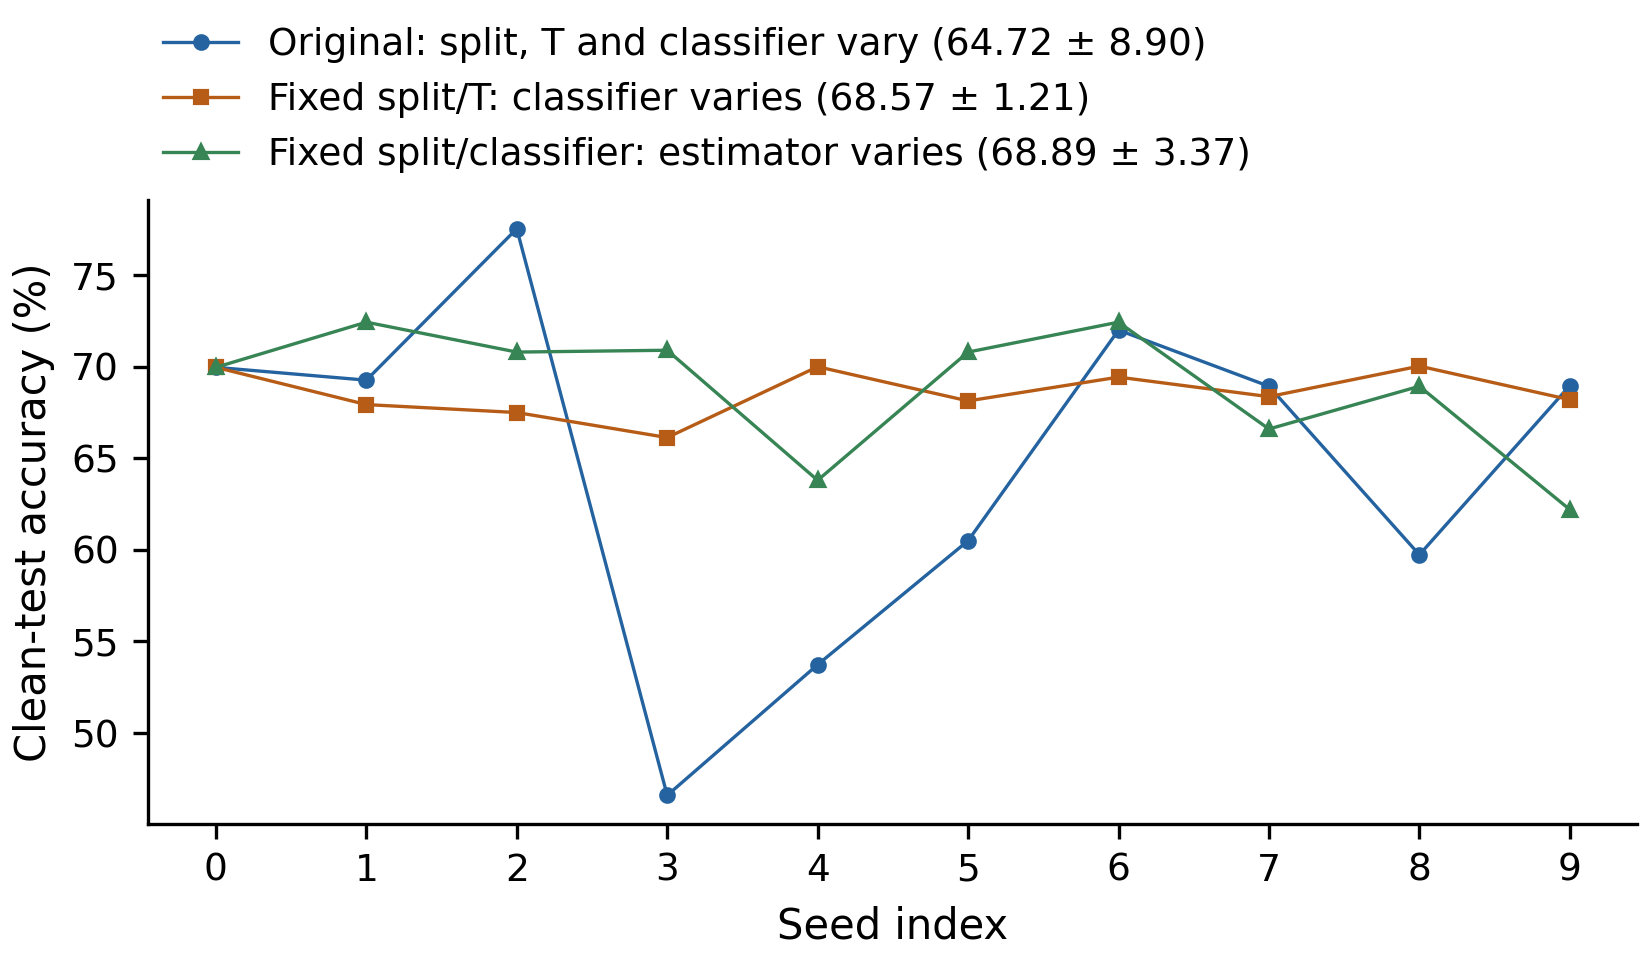
\includegraphics[width=\linewidth]{images/cifar_control_variability.png}
\caption{CIFAR Forward4 randomness controls. Legends give mean $\pm$ population SD over ten settings. Fixed-fold arms hold either the matrix or classifier seed constant; seed 0 is shared with the original experiment.}
\label{fig:cifar}\end{figure}
With split and matrix fixed, varying classifier randomness gives $68.57\pm1.21\%$. Varying the estimator while fixing split and classifier seed gives $68.89\pm3.37\%$, spanning 62.20--72.43\%. Estimator randomness therefore produces greater conditional variability on this reference fold. Both arms vary less than the original $64.72\pm8.90\%$, suggesting that split changes and interactions also merit investigation. This comparison cannot assign additive variance shares or establish that the same ranking holds on weaker folds.

Balanced test classes contain 1,000 examples each. Original Forward4 mean class recalls are 56.72, 65.53 and 71.92\%; Reweight-R gives 52.59, 69.78 and 74.66\%. The small aggregate R14 advantage therefore combines worse class-0 recall with improvements elsewhere. Seed 3 is weak across all classes (Forward: 41.3/54.6/43.9\%), whereas seed 4 particularly struggles with class 1 (25.7\%).

\clearpage
\section{Interpretation and limitations}
The known transitions are nonsingular but have spectral condition numbers approximately 1.64 and 10. For $T_{0.6}=0.1I+0.3\mathbf1\mathbf1^\top$, $q_i-q_j=0.1(p_i-p_j)$: observed class contrasts shrink tenfold. Avoiding explicit inversion does not remove weak supervision. Conversely, known-matrix importance weights satisfy $p_s/([pT]_s+\epsilon)\leq1/T_{ss}$, bounded by 1.43 or 2.5; unbounded weights are not the explanation here.

Joint noisy likelihood does not identify both components without further assumptions: $q=pT$ also admits $q=qI$. Known-matrix revision moves away from ground truth (mean Frobenius changes 0.0122/0.0156), so classification gains cannot establish better transition recovery. The fixed-matrix control directly tests the revision mechanism: almost all of the noise-0.3 improvement can be obtained by continuing optimization without learning a new matrix. The smaller, uncertain revision gains elsewhere should not be presented as evidence that the corruption process was recovered.

Epoch matching does not equate learning-rate schedules or exact computational cost. CIFAR controls use one reference fold and Forward4, not a complete variance decomposition for both classifiers. Calibration checks are not independent of prior checkpoint selection. Ten paired runs and a reused fixed test set quantify training variability conditional on these data, not uncertainty over new test populations. The class-conditional model can also fail under instance-dependent errors.

\section{Conclusion}
Forward and Reweight-R classify the known-noise datasets accurately, but their ranking depends on optimization budget. Forward14 reaches 99.08\% on FashionMNIST0.3; independent revision benefits are not established in the matched-checkpoint comparisons. Larger anchor averages reduce known-matrix error, whereas global temperature scaling does not reliably repair posterior-tail bias. CIFAR controls identify estimator randomness as an important conditional source of instability, alongside remaining split and interaction effects. Future work should test additional reference folds and calibrators that target anchor-tail probabilities, and select estimator settings using noisy validation rather than clean-test accuracy.

\section{Team contributions}
\textbf{Vaibhavi Shivanna:} robust losses, classifiers, training and revision. \textbf{Nihira Sharma:} data loading, preprocessing, splitting, estimation and visualizations. \textbf{Subaial Awan:} evaluation, verification, experiments and result analysis. \textbf{Shared:} integration, interpretation, report writing and final checks.

\clearpage
\appendix
\section{Reproduction and runtime}
Place the three raw \texttt{.npz} datasets in \texttt{code/data/}; only \texttt{.gitkeep} is shipped. From \texttt{code/} with Python 3.12:
\par\smallskip\noindent\begin{minipage}{\linewidth}\small\begin{verbatim}
python -m pip install -r requirements.txt
python -m pytest -q tests
python run_evaluation.py --runs 10 --workers 4 --threads 1 \
  --out reproduced_results
python verify_evaluation.py --results reproduced_results
python run_report_controls.py --baseline reproduced_results \
  --out report_controls --runs 10 --workers 4 --threads 1
python summarize_report_controls.py --baseline reproduced_results \
  --controls report_controls --out report_tables \
  --assets ../ASSETS/feedback_update
\end{verbatim}\end{minipage}\par\smallskip
Use fresh output folders after source/configuration changes. The canonical evaluation previously measured 58m 33.20s; the additional controls took \SupplementRuntime, separately measured. 53 tests pass; saved predictions independently reproduce reported accuracies. A one-repetition functional check uses \texttt{--runs 1}; final tables require all ten. Original runtime evidence uses an eight-logical-CPU ARM64 Mac, Python 3.12.2, NumPy 1.26.4 and PyTorch 2.11.0. Installation and verification are outside the quoted training-runtime scope.

\clearpage
\bibliographystyle{unsrt}\bibliography{references}
\end{document}
